\section{Dynamic typing}

\subsection{Dynamic typing}

\subsubsection{Variables, Object and References}

\textbf{As you know, Python is dynamically typed}
\begin{itemize}
	\item that is, there is no need to really explicit it
	\begin{lstlisting}[language=Python]
	>>> a = 42
	\end{lstlisting}
	\item Three separate concepts behind that assignment:
	\begin{itemize}
		\item \textbf{variable creation}, python works out names in spite of the (possibile) content
		\item \textbf{variable types}, no type associated to the variable name, type lives with the object
		\item \textbf{variable use} the name is replaced by the object when used in an expression
	\end{itemize}
\end{itemize}

\begin{lstlisting}[language=Python]
>>> a = 42
\end{lstlisting}
	
\textbf{What happens inside?}
\begin{itemize}
	\item Create an object to represent the value 42
	
	Objects are pieces of allocated memory
	
	\item Create the variable a, if it does not exist yet;
	
	Variables  are entries in a system table with spaces for links to objects
	
	\item Link the variable a to the new object 42
	
	References are automatically followed pointers from variables to objectsSS
\end{itemize}

\begin{center}
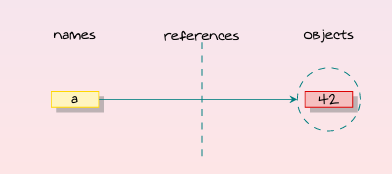
\includegraphics[scale=0.7]{1-variables-object-and-references}
\end{center}

\subsubsection{Types live with objects, not varables}

\begin{lstlisting}[language=Python]
>>> a = 42     # it's an integer
>>> a = 'spam' # now, it's string
>>> s = 3.14   # now, it's a floating point
\end{lstlisting}

\textbf{Coming from typed languages programming}

This lokks as the type of the name a changes

\textbf{Of course, this is not true. In python}

\begin{center}
Name have no types
\end{center}

\textbf{We simply changed the variable reference to a different object}

\textbf{Objects know what type they have}

Each object has an header field that tags it with its type

\textbf{Because objects know their type, variables don't have to}


\subsubsection{Object are garbage collected}

\textbf{What happens to the referenced object when the variable is reassinged?}

\begin{lstlisting}[language=Python]
>>> a = 42     
>>> a = 'spam'  # Reclaim 42 now (unless referenced elsewhere)
>>> s = 3.14    # Reclaim 'spam' now
>>> a = [1,2,3] # Reclaim 3.14 now
\end{lstlisting}

\textbf{The space held by the referenced object is reclaimed (garbage collected)}

If it is not referenced by any other name or object

Automatic garbage collection implies less bookkeeping code

\subsubsection{Shared references}

\textbf{What happens when a name changes its reference and the old valueis still referred?}

\begin{center}
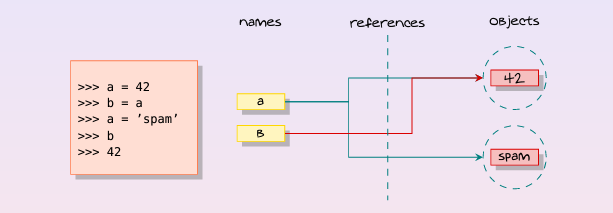
\includegraphics[scale=0.7]{2-shared-references}
\end{center}

\textbf{Is this still the same?}

\begin{lstlisting}[language=Python]
>>> a = [1,2,3]  
>>> b=a
>>> b[1]='spam'
>>> b
[1, 'spam', 3]
>>> a
[1, 'spam', 3]
\end{lstlisting}

\subsubsection{References \& Equality}

\textbf{Two ways to check equality}:

\begin{itemize}
	\item == (equality) and
	item is (object identity)
\end{itemize}

\begin{lstlisting}[language=Python]
>>> L=[1,2,3]
>>> M=[1,2,3]
>>> N=L
>>> L==M L is M
(True, False)
>>> L==N, L is N
(True, True)
\end{lstlisting}

\textbf{But...}

\begin{lstlisting}[language=Python]
>>> X = 42
>>> Y = 42
>>> X == Y, X is Y
(True, True)
\end{lstlisting}


\textbf{Small integers and dome other constant object are cached}

\begin{lstlisting}[language=Python]
>>> import sys
>>> sys.getrefcount(42)
10
>>> sys.getrefcount([1, 2, 3])
1
\end{lstlisting}

\subsubsection{References \& Passing Arguments}

\textbf{Argument are passed \textit{value}}

\begin{lstlisting}[language=Python]
X = 42
L = [1, 2, 3]

def fake_mutable(i,l):
	i = i * 2
	l[1] = '?!?!'
	l = {1, 3, 5,7 }
\end{lstlisting}

\begin{lstlisting}[language=Python]
>>> from args import fake_mutable, X, L
>>> print("X :- {0} \t L :- {1}".format(X,L))
X :- 42    L :- [1, 2, 3]
>>> fake_mutable(X,L)
>>> print("X :- {0} \t L :- {1}".format(X,L))
X :- 42    L :- [1, '?!?!', 3]
\end{lstlisting}

\textbf{Collections but tubìples are passed \textit{by refernece}}

\begin{lstlisting}[language=Python]
>>> L = [1, 2, 3]
>>> fake_mutable(X, L[:])
>>> print("X :- {0} \t L :- {1}".format(X,L))
X :- 42    L :- [1, 2, 3]
\end{lstlisting}

\textbf{Global values are immutalbe as wal, to vhange them use \textit{global}}

\begin{lstlisting}[language=Python]
def mutable():
	global X, L
	X = X*2
	L[1] = '?!?!'
	L = {1, 3, 5, 7}
if __name__ == "__main__":
mutable()
print("X :- {0} \t L :- {1}".format(X,L))
\end{lstlisting}

\begin{lstlisting}[language=Python]
X :- 84 L :- {1, 3, 5, 7}
\end{lstlisting}

\subsection{Closures in Action}

\subsubsection{Curring}

\(f(x, y) = \frac{y}{x} \xRightarrow{f(2, 3)} g(y) = f(2, y) = \frac{y}{2} \xRightarrow{g(3)} g(3) = \frac{3}{2}\)

\begin{lstlisting}[language=Python]
def make_currying(f, a):
	def fc(*args):
		return f(a, *args)
	return fc
	
def f2(x, y):
	return x+y
	
def f3(x, y, z):
	return x+y+z

if __name__ == "__main__":
	a = make_currying(f2, 3)
	b = make_currying(f3, 4)
	c = make_currying(b, 7)
	print("(cf2 3)({0}) :- {1}, (cf3 4)({2},{3}) :- {4}".format(1,a(1),2,3,b(2,3)))
	print("((cf3 4) 7)({0}) :- {1}".format(5,c(5)))
\end{lstlisting}


\begin{lstlisting}[language=Python]
(cf2 3)(1) :- 4, (cf3 4)(2,3) :- 9
((cf3 4) 7)(5) :- 16
\end{lstlisting}

Look at \textit{partial} in \textit{functools}
